\section{Implementation}
\subsection{Automation}
In the project, Ansible \cite{ansible} supports the deployment of AWS EC2 instances for Producer, Broker, RESTful API, Jenkins, and Web Application.
Then, Kubernetes \cite{kube} manages the deployment of the Producer, Broker, and RESTful API services.
Ansible managed the Jenkins and Web Application services, as they are less coupled to the rest of the services. 

\subsection{Producer}
The producer in our architecture was implemented as a background scheduler which iterated through a list of weather stations,
sending GET requests to the weatherbit API for the current weather. 
The producer then sent encoded topics to the Kafka broker.

\subsection{Broker}
The broker was implemented with Kafka \cite{kreps2011kafka} and Zookeeper \cite{hunt2010zookeeper}.

\subsection{Continuous Integration and Deployment}
Continuous integration and deployment was implemented through a containerized Jenkins instance \cite{jenkins}.

\subsection{RESTful API}
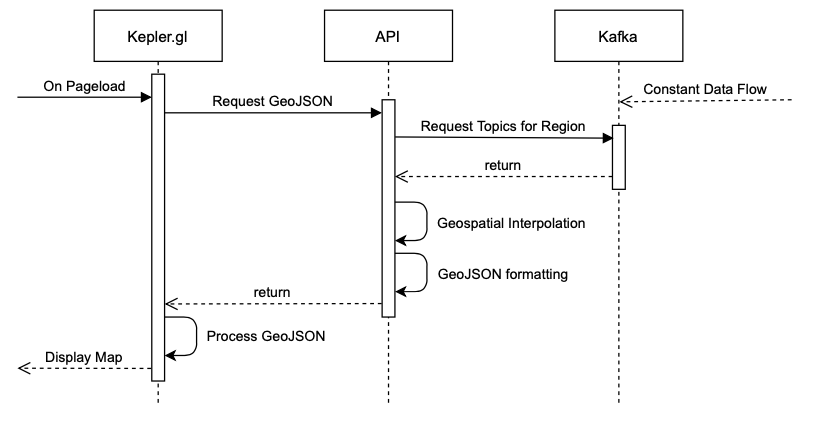
\includegraphics[width=\linewidth]{figures/Frontend_Flow.png}
In our API implementation, we used Flask, a python framework that allows us to build a simple API to interact with our web client and the Kafka brokers.
To interpolate, we use custom logic and SciPy to fill in the sparsity of the data.
The logic of the API scales with the size of the region requested from the front-end service.

\subsection{Web Application}
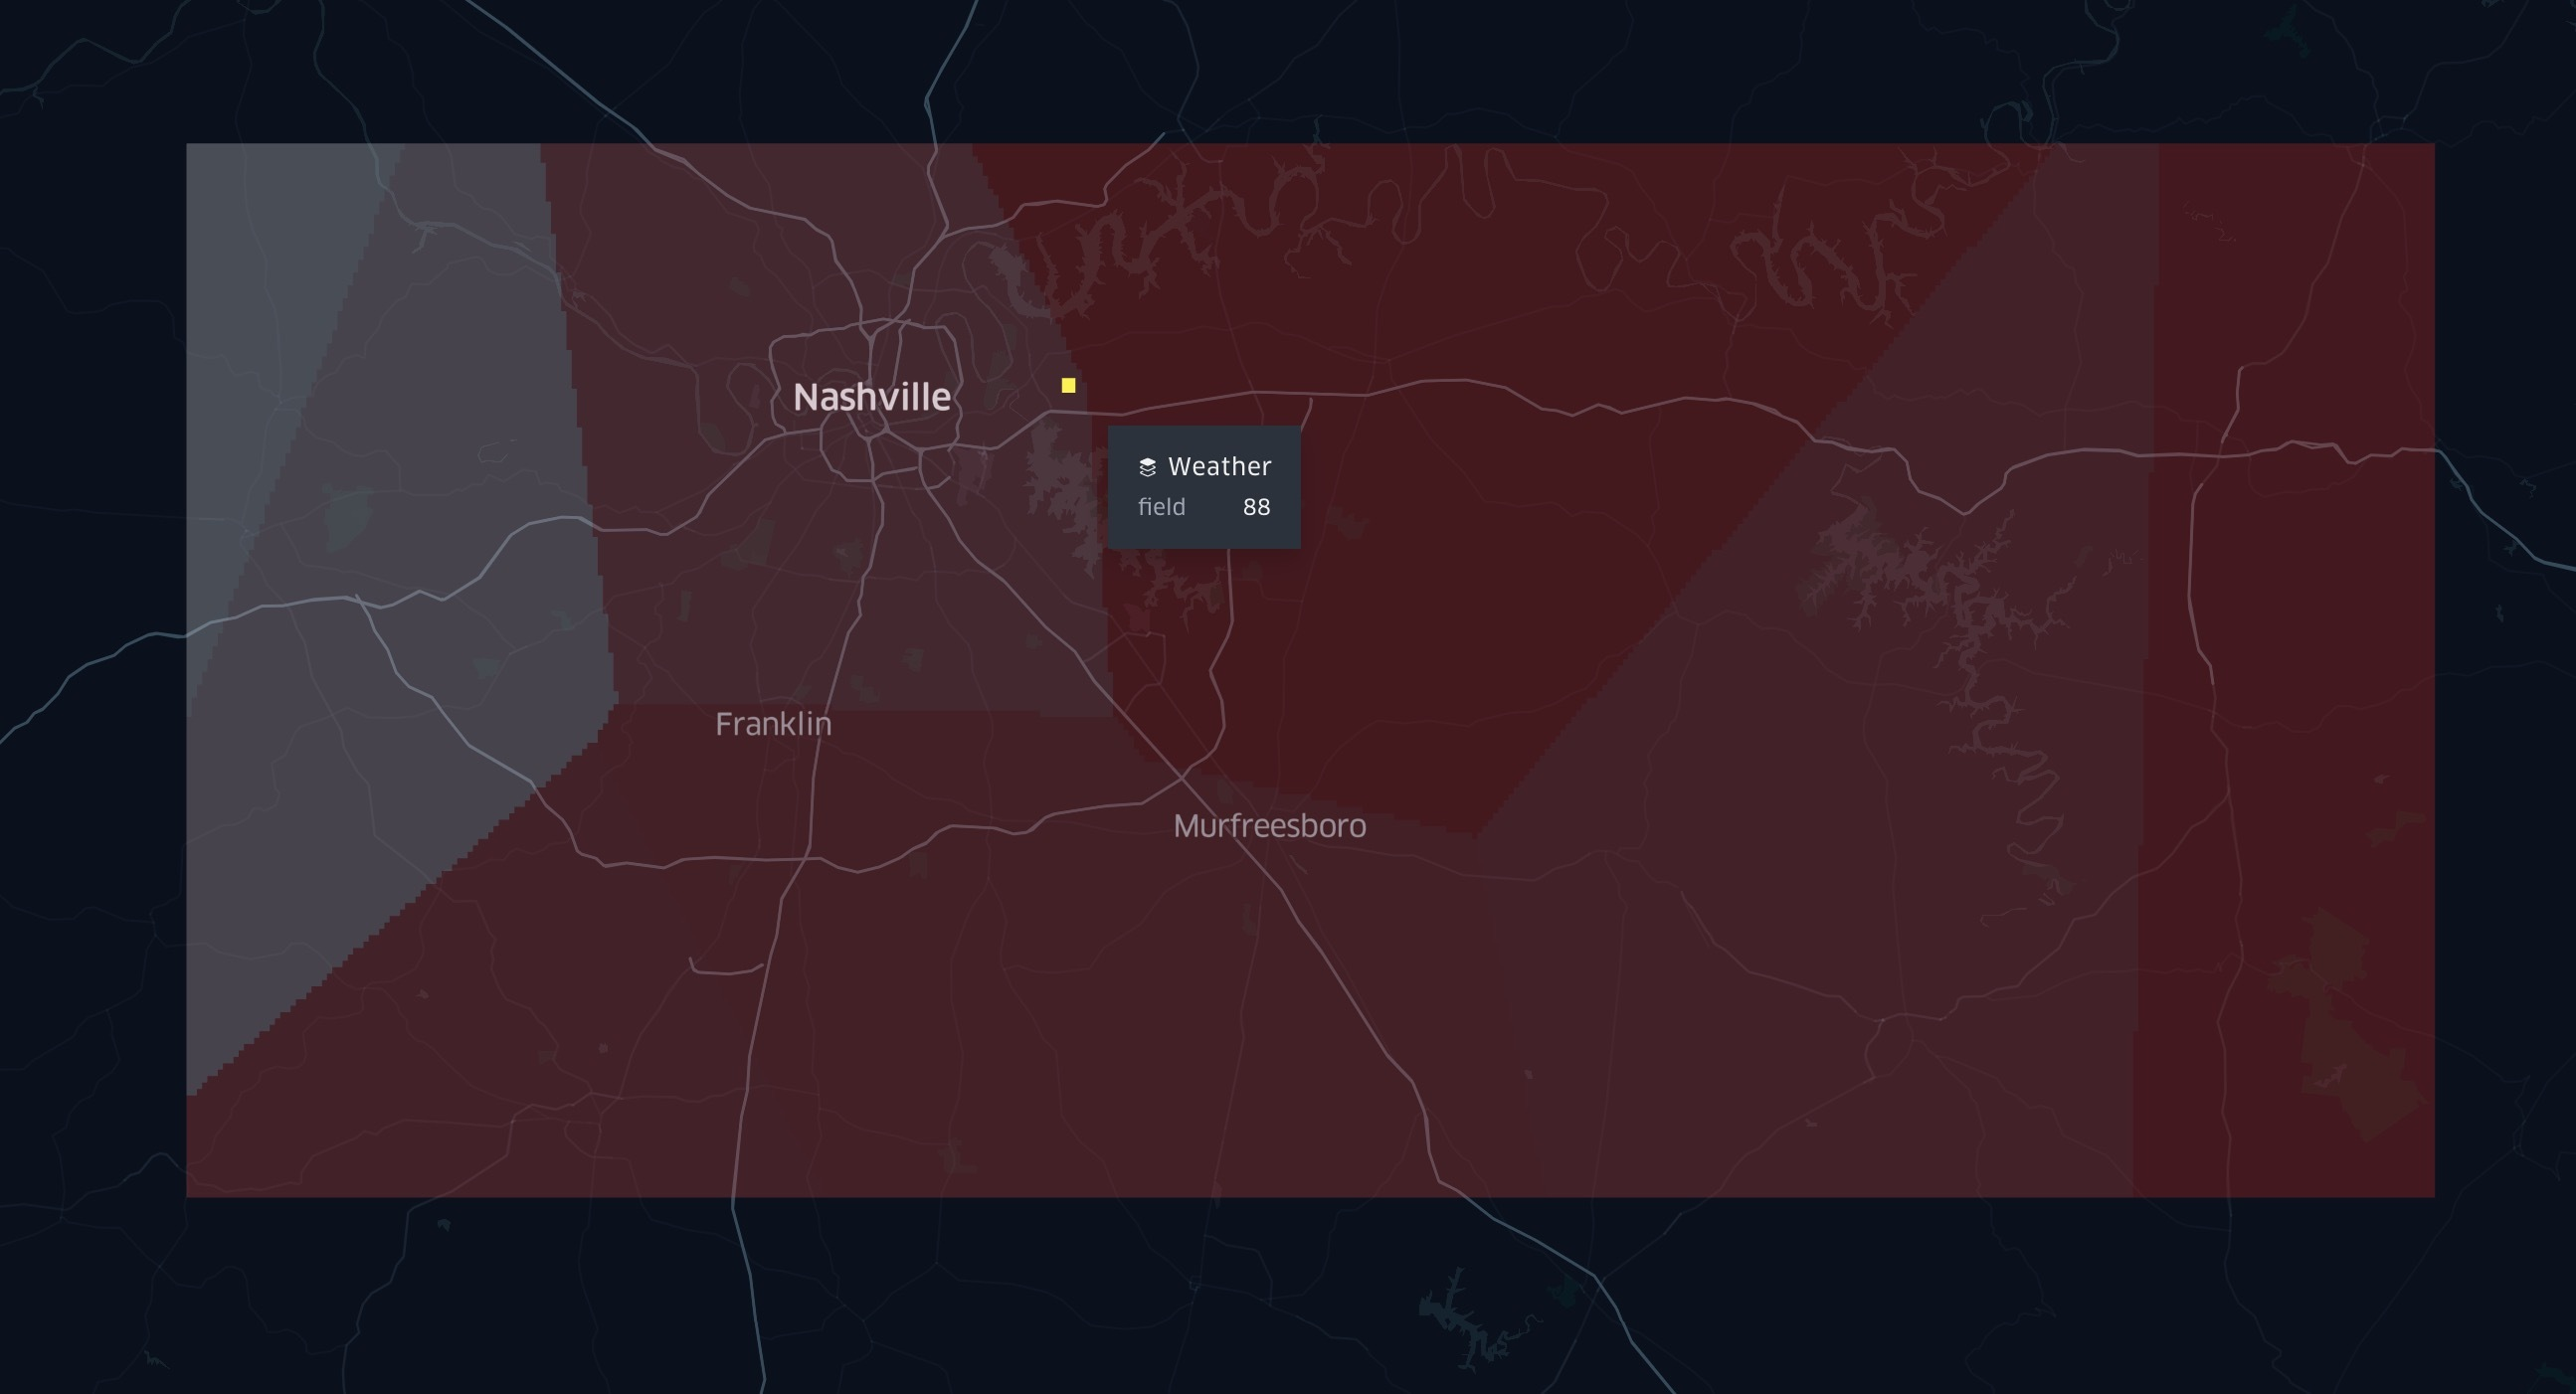
\includegraphics[width=\linewidth]{figures/dashboard.jpg}
For the dashboard, we used kepler.gl, which is a powerful open-source geospatial toolbox. It has libraries that work directly with the React web framework, making it possible to host our live data visualizations on a website. 
\cite{kepler}
The web application was configured from a \href{https://github.com/keplergl/kepler.gl/tree/master/examples/node-app}{kepler.gl example node app},
with modifications to connect to our API and tweaks to the visualization settings for a better user experience. 

Upon application initialization, a repeating interval of 15 minutes is set, at which point the app requests data from the API. The API returns a list of polygons whose shapes are dictated by coordinates. These polygons, rectangles in this example, are also assigned a value relating to a field provided by weatherbit. We chose to display relative humidity in particular as we found this to have the most variance in the greater Nashville area. To make the visualization more interesting, the app applies color gradient to the polygons; higher relative humidity results in darker, deeper reds.